% ================================================================
%  DSC 208R -- Data Management for Analytics
%  Data Parallelism (Part 1): Comprehensive Review
%  Source: "Data Engineering for ML -- Data Parallelism Part 1"
% ================================================================
\documentclass[11pt]{article}

% -------------------- Packages --------------------
\usepackage[utf8]{inputenc}
\usepackage{amsmath,amssymb,amsfonts}
\usepackage{graphicx}
\usepackage{booktabs}
\usepackage{tikz}
\usetikzlibrary{positioning}
\usepackage{pgfplots}
\usepackage{enumitem}
\usepackage{listings}
\usepackage{hyperref}
\usepackage{caption}
\pgfplotsset{compat=1.17}

% -------------------- Listings --------------------
\lstset{
  basicstyle=\ttfamily\small,
  keywordstyle=\bfseries,
  commentstyle=\itshape,
  showstringspaces=false,
  frame=single,
  breaklines=true
}

% -------------------- Document --------------------
\begin{document}

\begin{center}
  {\LARGE\bfseries Data Parallelism (Part 1)}\\[2mm]
  {\large Comprehensive Review}\\[1mm]
  {\normalsize DSC 208R -- Parallel Data Processing and the Cloud}
\end{center}
\vspace{-0.6em}\hrule\vspace{0.9em}

\tableofcontents
\newpage

% ================================================================
\section{Motivation}

Data parallelism partitions large data sets across multiple workers so that each worker operates on its own shard.  This strategy is the backbone of scalable systems that handle data sets too large for a single machine.:contentReference[oaicite:0]{index=0}

% ================================================================
\section{System Context}

Classical multi-node architectures are shared-nothing, shared-memory, and shared-disk.  Data parallelism aligns best with \emph{shared-nothing} clusters, where each node owns its local shard and communicates with others only when necessary.:contentReference[oaicite:1]{index=1}

\subsection*{Shared-Nothing Cluster Illustration}

\begin{figure}[h]
  \centering
  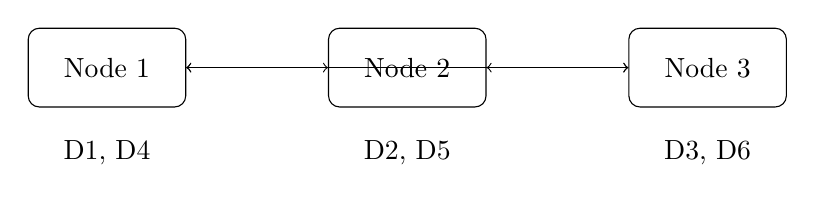
\begin{tikzpicture}[
    node/.style={draw,rounded corners,minimum width=2cm,minimum height=1cm},
    yshift=-0.3cm
  ]
    \node[node] (w1) {Node 1};
    \node[node,right=1.8cm of w1] (w2) {Node 2};
    \node[node,right=1.8cm of w2] (w3) {Node 3};

    \node[below=0.3cm of w1] {D1, D4};
    \node[below=0.3cm of w2] {D2, D5};
    \node[below=0.3cm of w3] {D3, D6};

    \draw[<->] (w1) -- (w2);
    \draw[<->] (w2) -- (w3);
    \draw[<->] (w1) -- (w3);
  \end{tikzpicture}
  \caption{Shared-nothing cluster with six data shards.}
\end{figure}

% ================================================================
\section{Row-Wise Partitioning Strategies}

For \(k\) workers the main schemes are: contentReference[oaicite:2]{index=2}
\begin{enumerate}[itemsep=0pt]
  \item Round-robin: tuple \(i\) goes to worker \((i \bmod k)\).
  \item Hash: apply a hash to one or more attributes.
  \item Range: assign contiguous key ranges to workers.
\end{enumerate}

\paragraph{Notes.}
Hashing dominates SQL engines; range can accelerate range predicates; round-robin is simplest but ignores skew.

% ================================================================
\section{Replication for Fault Tolerance}

Replicating every shard (for example, three copies) improves durability and enables locality-aware scheduling at the cost of extra storage.:contentReference[oaicite:3]{index=3}

% ================================================================
\section{Column and Hybrid Layouts}

Single-node disk layouts generalize to clusters:contentReference[oaicite:4]{index=4}
\begin{itemize}[itemsep=0pt]
  \item Column layouts store each column (or group) across workers.
  \item Hybrid or tiled layouts combine row and column slicing.
\end{itemize}
Such layouts help workloads that read only a subset of columns.

% ================================================================
\section{Cluster Coordination Styles}

\begin{itemize}[itemsep=0pt]
  \item \textbf{Manager-worker} (centralized): one node assigns tasks.  Examples include Dask and Spark.:contentReference[oaicite:5]{index=5}
  \item \textbf{Peer-to-peer} (decentralized): workers coordinate directly, as in Horovod.:contentReference[oaicite:6]{index=6}
\end{itemize}

\begin{figure}[h]
  \centering
  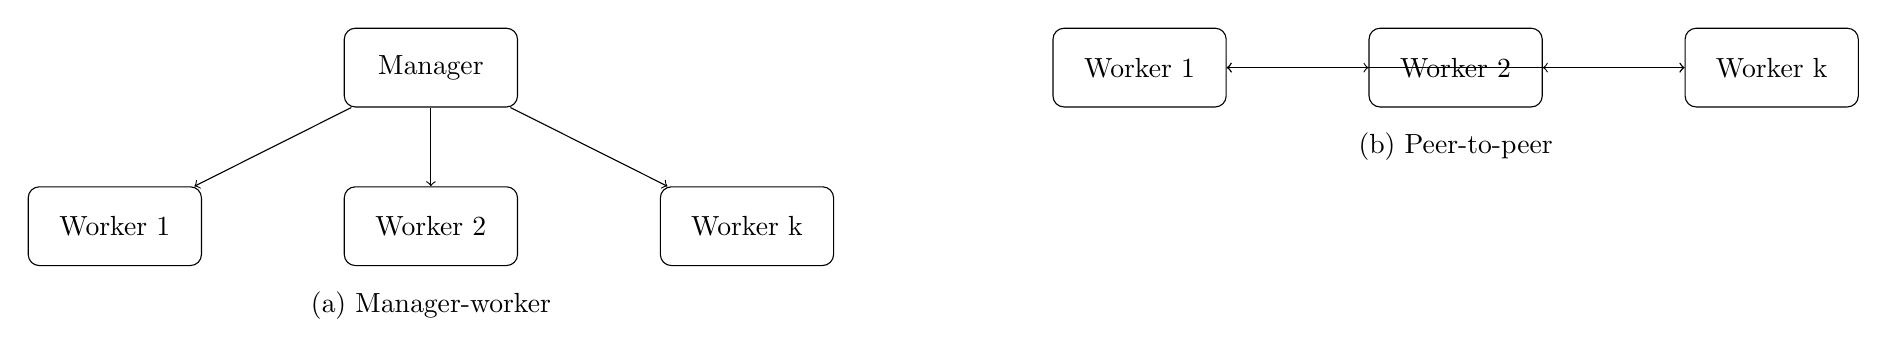
\begin{tikzpicture}[
    node/.style={draw,rounded corners,minimum width=2.2cm,minimum height=1cm}
  ]
    % Manager-worker
    \node[node] (mgr) {Manager};
    \node[node,below left=1cm and 1.8cm of mgr] (mw1) {Worker 1};
    \node[node,below=1cm of mgr] (mw2) {Worker 2};
    \node[node,below right=1cm and 1.8cm of mgr] (mwk) {Worker k};

    \draw[->] (mgr) -- (mw1);
    \draw[->] (mgr) -- (mw2);
    \draw[->] (mgr) -- (mwk);

    \node[draw=none,below=0.2cm of mw2] {(a) Manager-worker};

    % Peer-to-peer (shifted right)
    \begin{scope}[shift={(9,0)}]
      \node[node] (p1) {Worker 1};
      \node[node,right=1.8cm of p1] (p2) {Worker 2};
      \node[node,right=1.8cm of p2] (pk) {Worker k};

      \draw[<->] (p1) -- (p2);
      \draw[<->] (p2) -- (pk);
      \draw[<->] (p1) -- (pk);

      \node[draw=none,below=0.2cm of p2] {(b) Peer-to-peer};
    \end{scope}
  \end{tikzpicture}
  \caption{Two coordination styles for data-parallel clusters.}
\end{figure}

% ================================================================
\section{Pros and Cons}

\begin{itemize}[itemsep=0pt]
  \item \textbf{Pros}
    \begin{itemize}[itemsep=0pt]
      \item Horizontal scalability beyond one machine.
      \item Clear mental model: each worker processes local data.
      \item Works naturally with replication.
    \end{itemize}
  \item \textbf{Cons}
    \begin{itemize}[itemsep=0pt]
      \item Cross-shard joins and shuffles can dominate runtime.
      \item Skewed partitions lead to load imbalance.
      \item Coordination overhead grows with cluster size.
    \end{itemize}
\end{itemize}

% ================================================================
\section{Future Directions}

\begin{itemize}[itemsep=0pt]
  \item Adaptive, workload-aware partitioning rather than static hash or range.
  \item Dynamic replication levels driven by failure probability and data locality.
  \item Tighter integration with cloud object storage tiers for cost efficiency.
\end{itemize}

% ================================================================
\section*{Conclusion}

Data parallelism divides data across many workers so that each can process a shard in parallel.  The shared-nothing model with hash or range partitioning remains the default, but ongoing work targets smarter partitioning, adaptive replication, and better cloud integration.:contentReference[oaicite:7]{index=7}

\end{document}
